\section{Definitions and Notations}
We consider the problem as presented in \cite{gravitymachine}. The multi-objective 0-1 linear optimisation problems with $p$ objectives ($p$-01LP) considered can be formulated as follows:
\begin{align*}
    \min z(x)&=Cx\\
    \text{subject to } Ax &\leqq b\\
    x &\in \set{0,1}^n
\end{align*}
where
\begin{itemize}
    \item $x\in \set{0,1}^n$, the vector of $n$ binary variables $x_j, j=1,\ldots,n$;
    \item $A\in\mathbb{R}^{m\times n}$, the $m$ constraints $A_ix \leq b_i, \; i=1,\ldots,m$ and $b\in \mathbb{R}^m$;
    \item $C \in \mathbb{R}^{p\times n}$, the objective matrix where $p \geq 2$;
    \item $X:=\set{x\in\set{0,1}^n\mid Ax \leqq b} \subseteq \mathbb{R}^n$, the set of feasible solutions, with $\mathbb{R}^n$ the decision space;
    \item $Y:=\set{Cx\mid x \in X}\subseteq\mathbb{R}^p$, the outcome set, with $\mathbb{R}^p$ the objective space.
\end{itemize}
Thereafter, $p$ is usually meant to be equal to $2$ (\textit{e.g.} we consider the bi-objective class of problems).
\begin{definition}[\cite{MultOptEhrgott}]
A feasible solution $\hat{x}\in\mathcal{X}$ is called efficient or Pareto optimal if there is no other $x \in \mathcal{X}$ such that $f(x)\leq f(\hat{x})$. If $\hat{x}$ is efficient, $f(\hat{x})$ is called nondominated point. If $x^1, x^2 \in \mathcal{X}$ and $f(x^1)\leq f(x^2)$ we say $x^1$ dominates $x^2$ and $f(x^1)$ dominates $f(x^2)$. The set of all efficient solutions $\hat{x} \in \mathcal{X}$ is denoted $\mathcal{X}_E$ and called the efficient set. The set of all nondominated points $\hat{y}=f(\hat{x})\in\mathcal{Y}$, where $\hat{x}\in\mathcal{X}_E$, is denoted $\mathcal{Y}_N$ and called the nondominated set.
\end{definition}
\begin{definition}[\cite{MultOptEhrgott}]
A feasible solution $\hat{x}\in \mathcal{X}$ is called weakly efficient (weakly Pareto optimal) if there is no $x\in \mathcal{X}$ such that $f(x)<f(\hat{x})$, \textit{i.e.} $f_k(x)<f_k(\hat{x})$ for all $k=1,\ldots,p$. The point $\hat{y}=f(\hat{x})$ is then called weakly nondominated. A feasible solution $\hat{x}\in\mathcal{X}$ is called strictly efficient (strictly Pareto optimal) if there is no $x\in\mathcal{X}$,$x\neq\hat{x}$ such that $f(x)\leqq f(\hat{x})$. The weakly (strictly) efficient and nondominated sets are denoted $\mathcal{X}_{wE}(\mathcal{X}_{sE})$ and $ \mathcal{Y}_{wE}$, respectively. 
\end{definition}

\begin{definition}[A lower bound set~\cite{boundssetsXGME}]
A lower bound set for $Y'$ is a subset $L \subseteq \mathbb{R}^p$
\begin{enumerate}
    \item For each $y\in Y'$ there is some $l\in L$ such that $l\leqq y$
    \item There is no pair $y\in Y',l\in L$ such that $y$ dominates $l$.
\end{enumerate}
\end{definition}
\begin{definition}[An upper bound set~\cite{boundssetsXGME}]
An upper bound set for $Y'$ is a subset $U \subset \mathbb{R}^p$
\begin{enumerate}
    \item For each $y\in Y'$ there is some $u\in U$ such that $y\leqq u$
    \item There is no pair $y\in Y',\in U$ such that $u$ dominates $y$.
\end{enumerate}
\end{definition}
%\pagestyle{empty}
\definecolor{ttfftt}{rgb}{0.2,1,0.2}
\definecolor{ffwwww}{rgb}{1,0.4,0.4}
\definecolor{qqttff}{rgb}{0,0.2,1}
\definecolor{qqqqff}{rgb}{0,0,1}
\definecolor{ttttff}{rgb}{0.2,0.2,1}
\definecolor{fftttt}{rgb}{1,0.2,0.2}
\definecolor{cqcqcq}{rgb}{0.75,0.75,0.75}
\begin{tikzpicture}[line cap=round,line join=round,>=triangle 45,x=10.0cm,y=10.0cm]
\draw [color=cqcqcq,dash pattern=on 2pt off 2pt, xstep=2.0cm,ystep=2.0cm] (-0.4,-0.2) grid (1.4,1.2);
\draw[->,color=black] (-0.4,0) -- (1.4,0);
\foreach \x in {-0.4,-0.2,0.2,0.4,0.6,0.8,1,1.2,1.4}
\draw[shift={(\x,0)},color=black] (0pt,2pt) -- (0pt,-2pt) node[below] {\footnotesize $\x$};
\draw[->,color=black] (0,-0.2) -- (0,1.2);
\foreach \y in {-0.2,0.2,0.4,0.6,0.8,1}
\draw[shift={(0,\y)},color=black] (2pt,0pt) -- (-2pt,0pt) node[left] {\footnotesize $\y$};
\draw[color=black] (0pt,-10pt) node[right] {\footnotesize $0$};
\clip(-0.4,-0.2) rectangle (1.4,1.2);
\fill[color=ttfftt,fill=ttfftt,fill opacity=0.1] (0,1) -- (1,1) -- (1,0) -- cycle;
\draw [line width=1.6pt,dash pattern=on 3pt off 3pt,color=ffwwww,domain=-0.4:1.4] plot(\x,{(--1-1*\x)/1});
\draw [color=ttfftt] (0,1)-- (1,1);
\draw [color=ttfftt] (1,1)-- (1,0);
\draw [color=ttfftt] (1,0)-- (0,1);
\begin{scriptsize}
\fill [color=fftttt] (0,0) circle (2.5pt);
\draw[color=fftttt] (0.05,0.04) node {$(0, 0)$};
\fill [color=ttttff] (0,1) circle (2.5pt);
\draw[color=ttttff] (0.05,1.04) node {$(0, 1)$};
\fill [color=qqqqff] (1,1) circle (2.5pt);
\draw[color=qqqqff] (1.05,1.04) node {$(1, 1)$};
\fill [color=qqttff] (1,0) circle (2.5pt);
\draw[color=qqttff] (1.05,0.04) node {$(1, 0)$};
\draw[color=ffwwww] (-0.59,1.67) node {$x + y = 1$};
\end{scriptsize}
\end{tikzpicture}

\begin{figure}
    \centering
    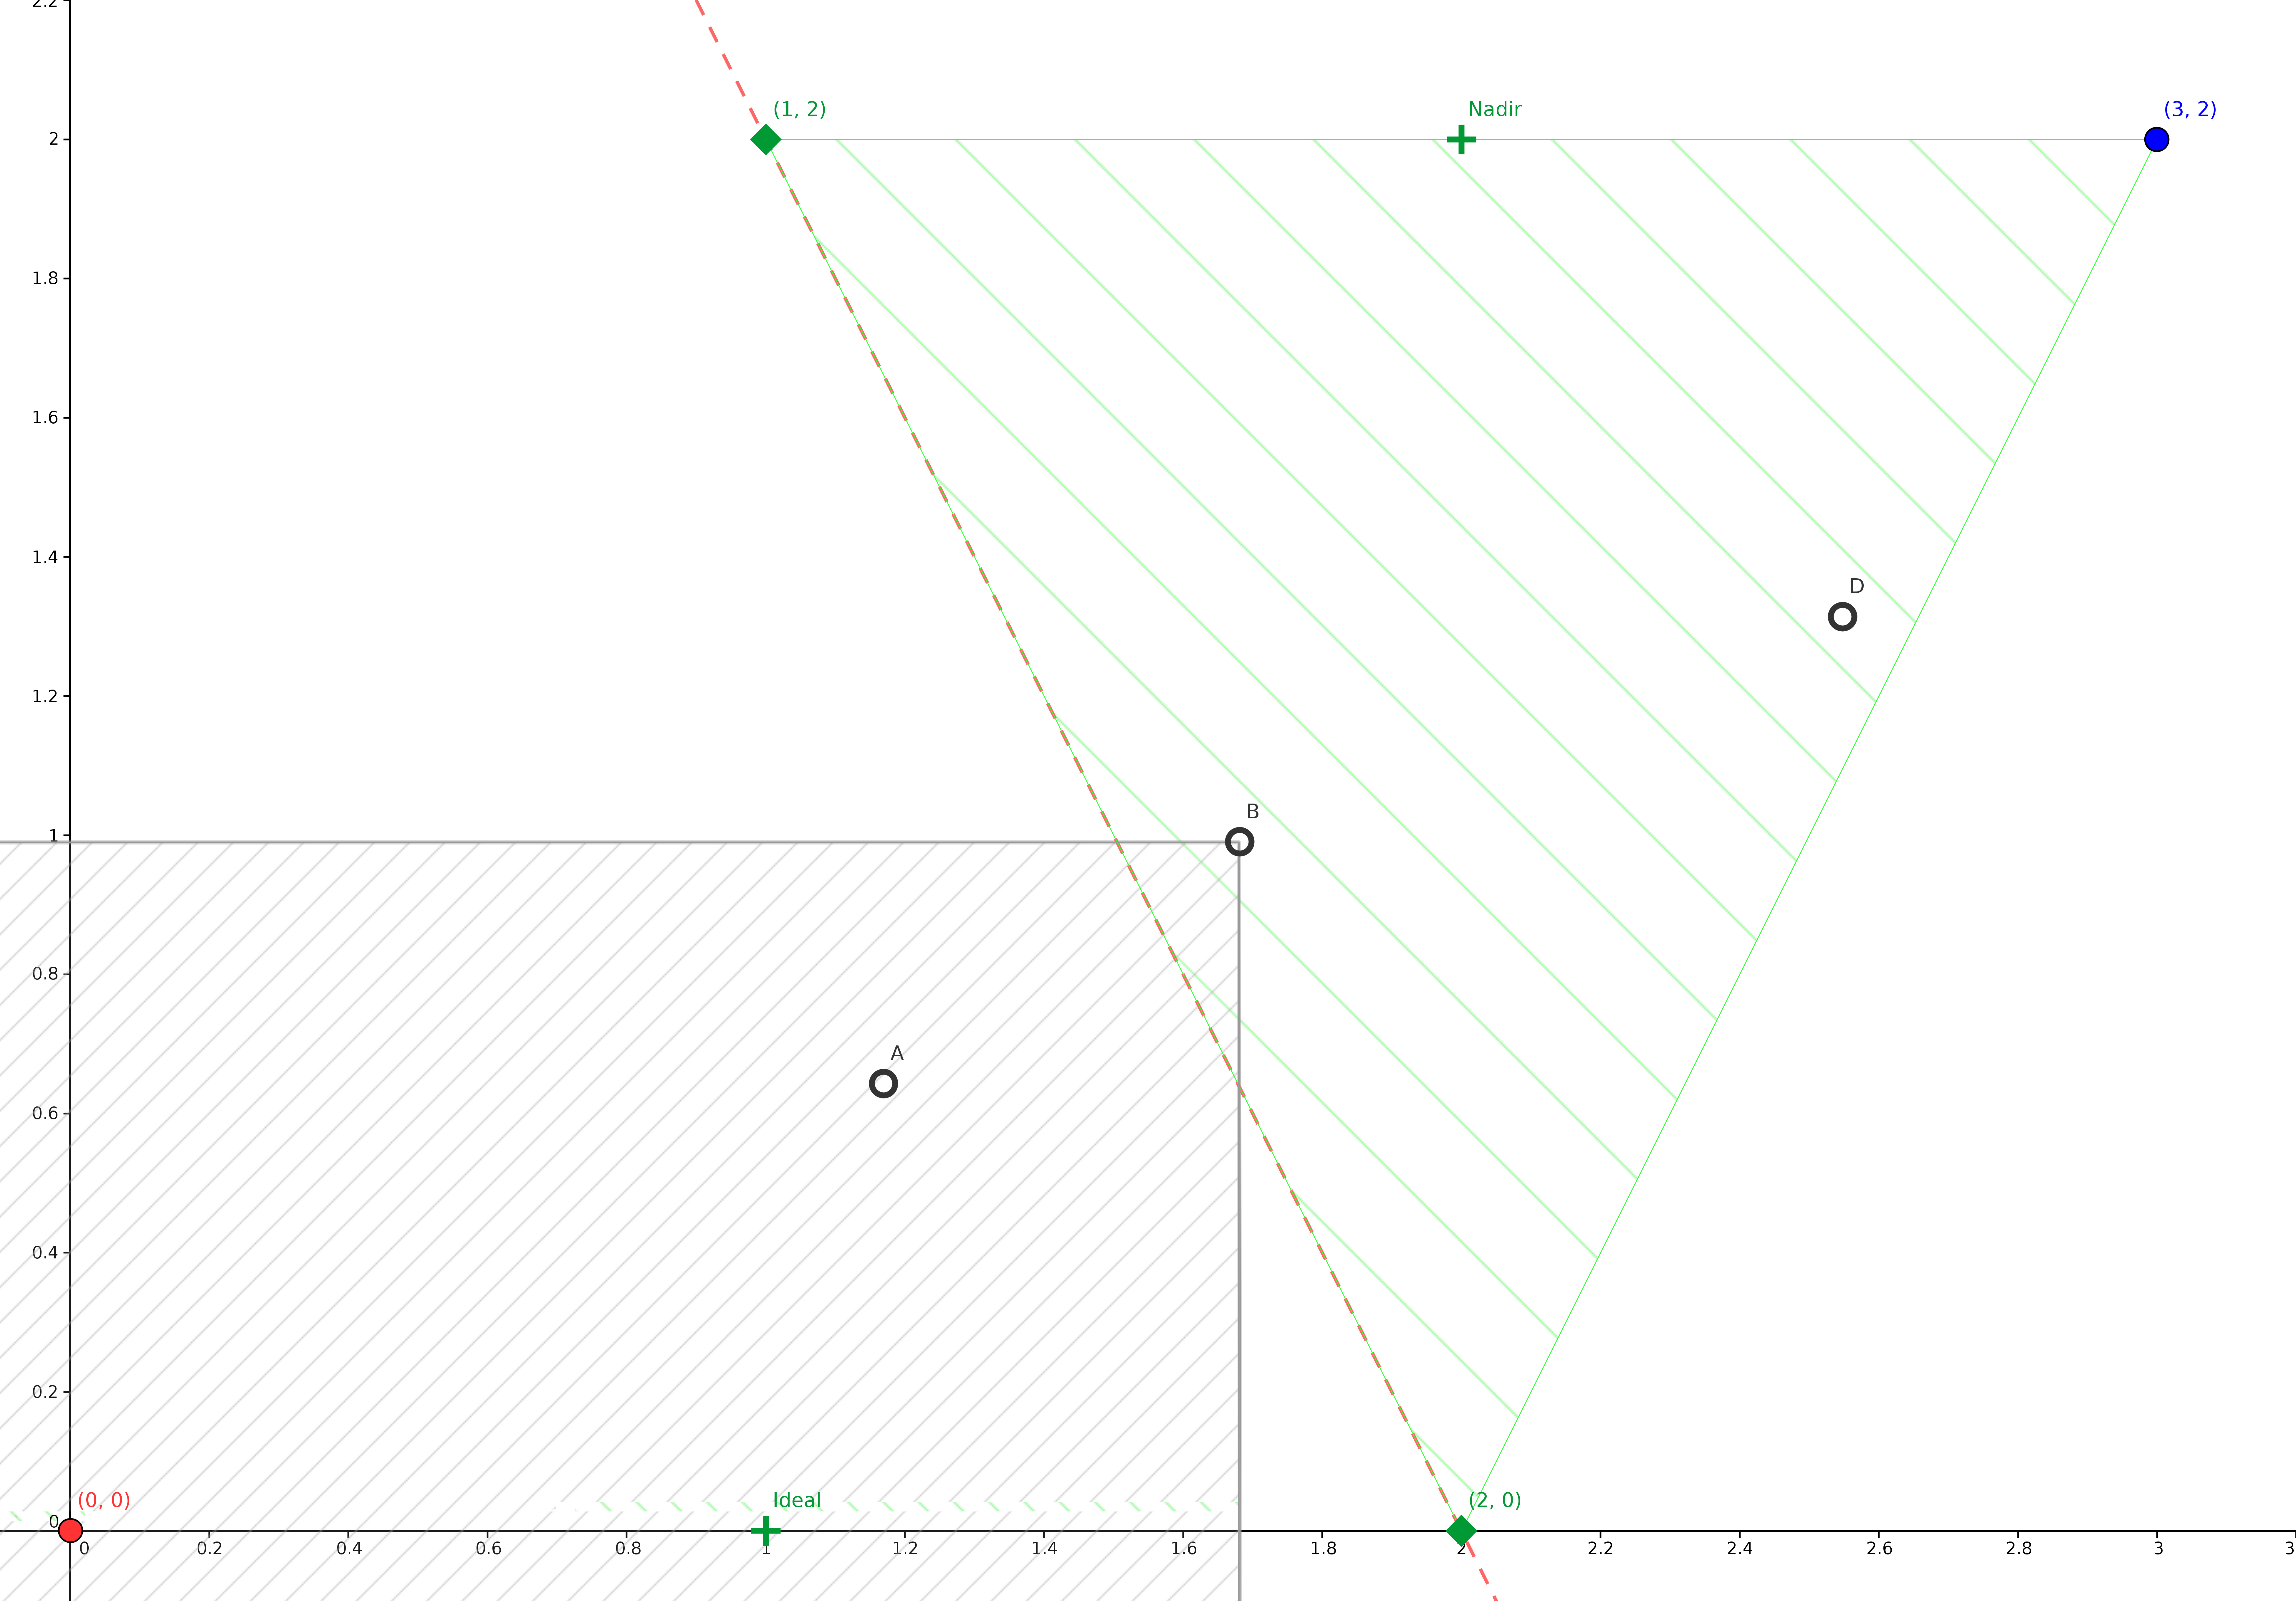
\includegraphics[scale=0.45]{figures_tikz/figure1_exempleCOST.png}
    \caption{Projection of the solution space onto the cost space}
    \label{fi:costspace}
\end{figure}